
\chapter{Emacs}
\label{cha:emacs}

Type all the \TeX\xspace commands is time consuming and error prone.
\keyword{Emacs} comes to the rescue. It can auto-fill the commands.

Emacs comes with a package for editing TeX and LaTeX files.
However, this package is extremely limited in its functionality.
A far better package called \keyword{AUC TeX} can help you write your papers efficiently.

Here is the Figure of using Emacs:
\begin{figure}[H]
  \centering
  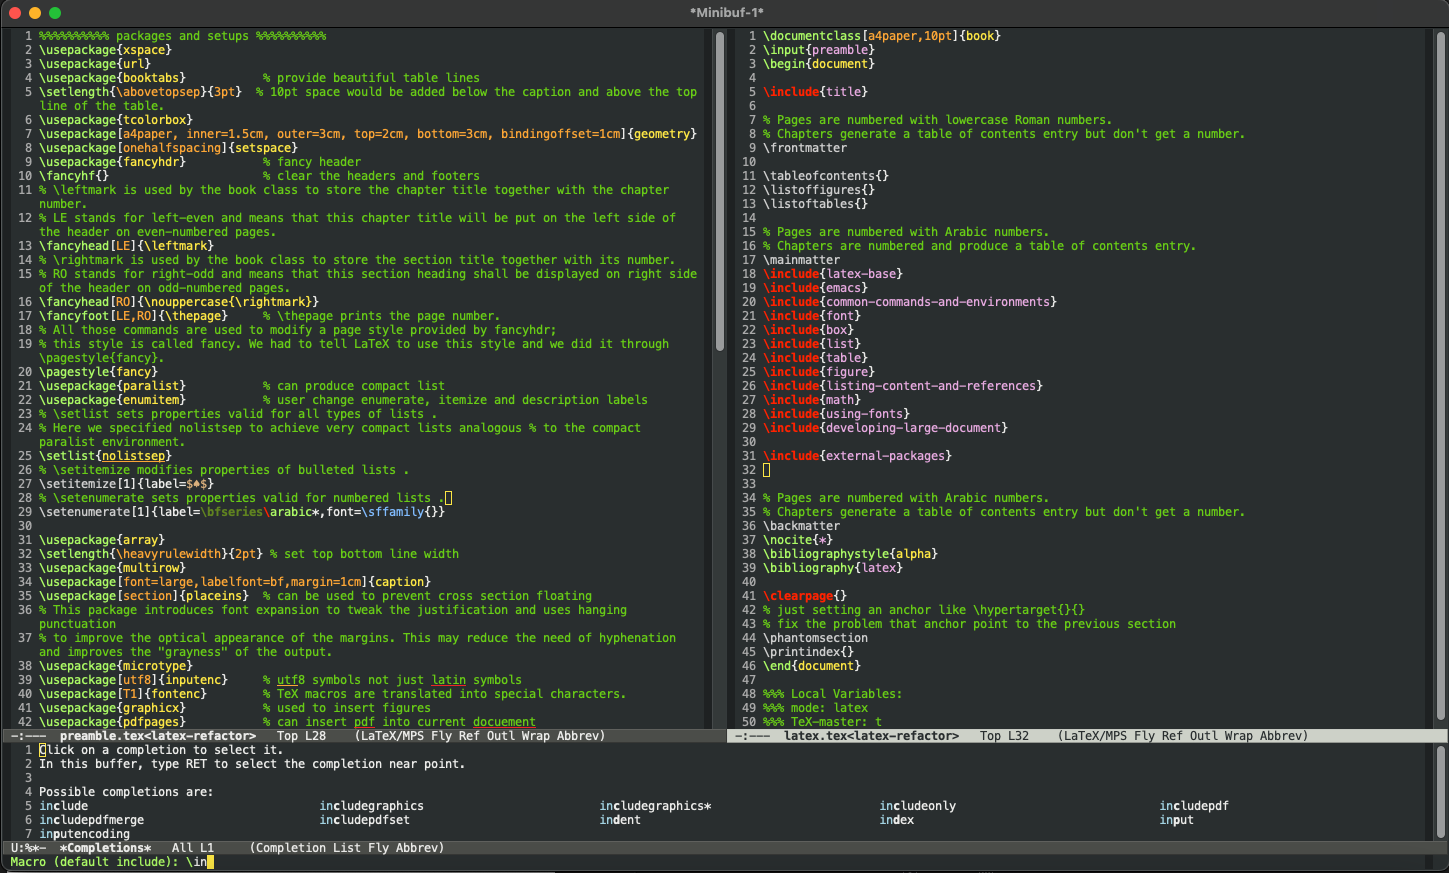
\includegraphics[width=\textwidth]{emacs}
  \caption{Emacs}
  \label{fig:emacs}
\end{figure}


%%% Local Variables:
%%% mode: latex
%%% TeX-master: "latex"
%%% End:
